\section{Extension framework measurements}

We describe in this section the results obtained with the extension framework described in the section \ref{sec:extension}.
First, the results are shown without any comments with tables and plots.
Later, we discuss the results by comparing them with the reference value.

\subsection{Measurement}

In the same way as with the reference value, the results are divided by boards.
The measurements made with the RE-Mote boards are first given, then the one made with Z1 board.
The Contiki measurements are displayed side-by-side with the RIOT OS one.

\subsubsection{RE-Mote measurements}
The table \ref{tab:extension-framework-remote}, the figure \ref{fig:extension-framework-contiki-remote} and the figure \ref{fig:extension-framework-riot-remote} show the measurement for Contiki and RIOT OS for the RE-Mote board.

\begin{table}[!ht]
  \centering
  \begin{tabular}{l|c|c}
                & Contiki  & RIOT \\ \hline
  Mean ($\mu$s) & 31.6162  & 17      \\
  Min  ($\mu$s) & 0        & 17      \\
  Max  ($\mu$s) & 457.7636 & 17     
  \end{tabular}
  \caption{extension approach measurements for Contiki and RIOT on the RE-Mote board}
  \label{tab:extension-framework-remote}
  \end{table}

\begin{figure}[!ht]
  \begin{minipage}{.45\textwidth}
      \centering
      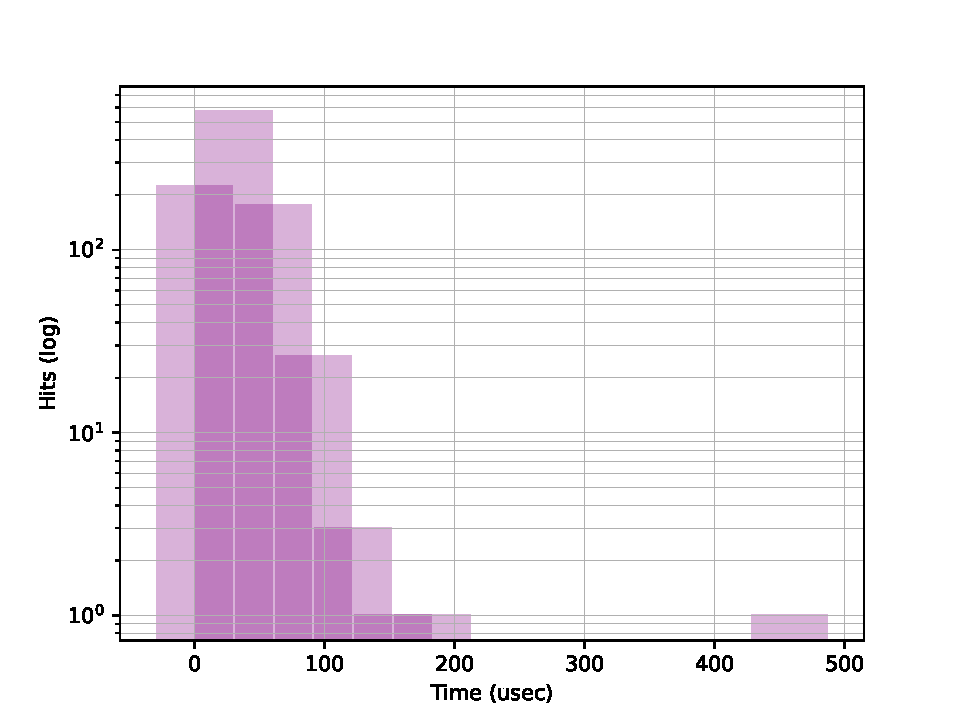
\includegraphics[scale=.4]{assets/extension-framework-contiki-remote.pdf}
      \caption{Extension framework distribution with Contiki on RE-Mote\label{fig:extension-framework-contiki-remote}}
  \end{minipage}\hfill
  \begin{minipage}{.45\textwidth}        
      \centering
      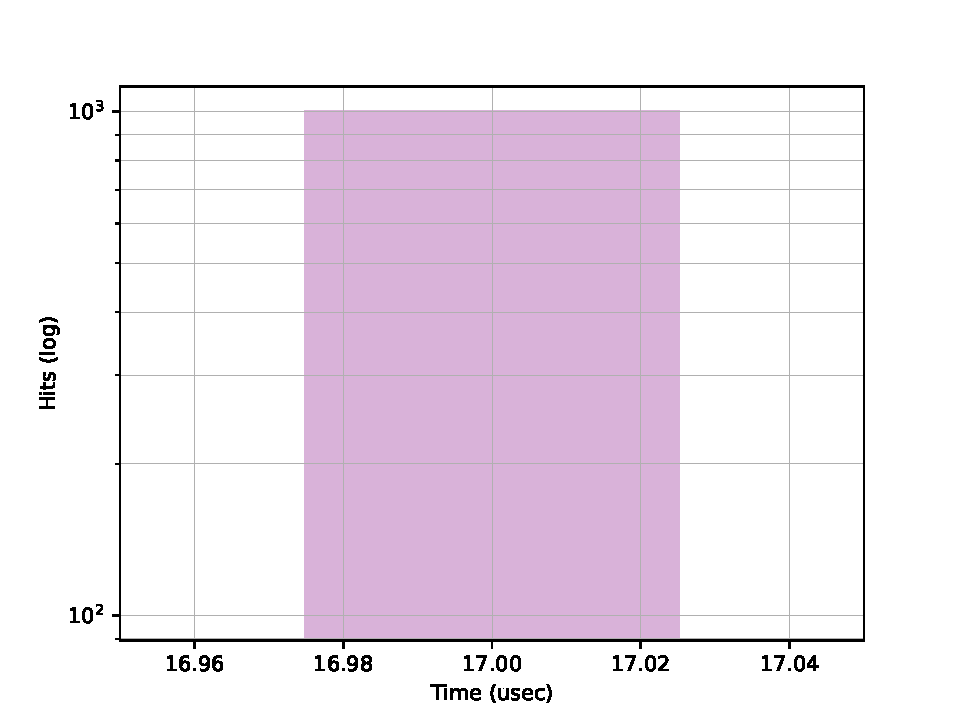
\includegraphics[scale=.4]{assets/extension-framework-riot-remote.pdf}
      \caption{Extension framework distribution with RIOT on RE-Mote\label{fig:extension-framework-riot-remote}}
  \end{minipage}
\end{figure}

\subsubsection{Z1 measurements}
The table \ref{tab:extension-framework-z1}, the figure \ref{fig:extension-framework-contiki-z1} and the figure \ref{fig:extension-framework-riot-z1} show the measurement for Contiki and RIOT OS for the Z1 board.

\begin{table}[!ht]
  \centering
  \begin{tabular}{l|c|c}
                & Contiki  & RIOT \\ \hline
  Mean ($\mu$s) & 90.5761  & 40.252      \\
  Min  ($\mu$s) & 30.5175  & 40      \\
  Max  ($\mu$s) & 976.5625 & 41     
  \end{tabular}
  \caption{extension approach measurements for Contiki and RIOT on the Z1 board}
  \label{tab:extension-framework-z1}
  \end{table}

\begin{figure}[!ht]
  \begin{minipage}{.45\textwidth}
      \centering
      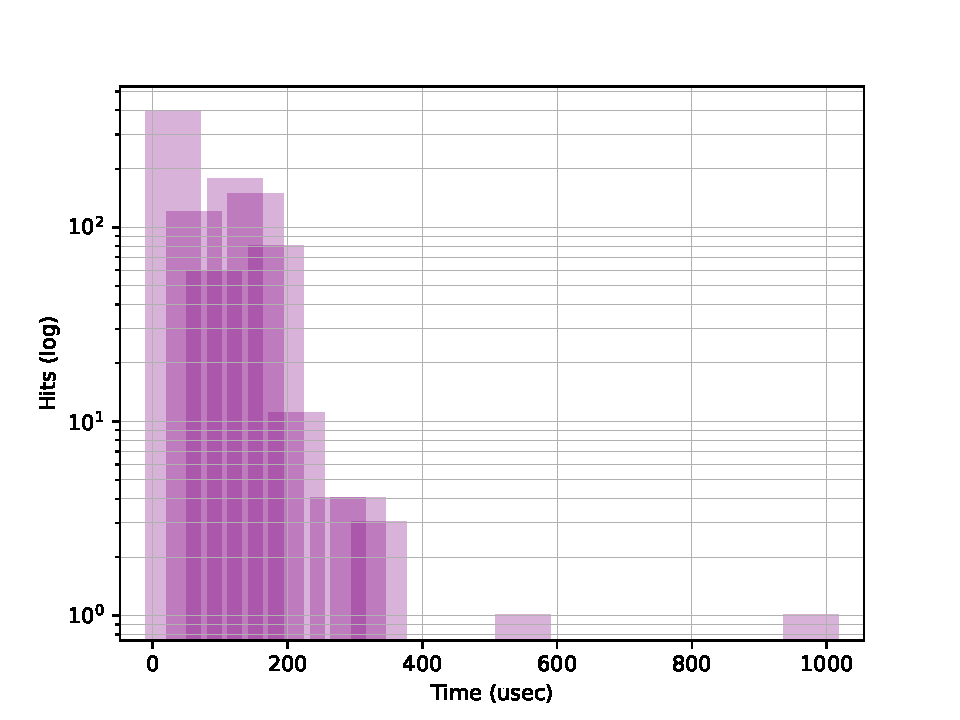
\includegraphics[scale=.4]{assets/extension-framework-contiki-z1.pdf}
      \caption{Extension framework distribution with Contiki on Z1\label{fig:extension-framework-contiki-z1}}
  \end{minipage}\hfill
  \begin{minipage}{.45\textwidth}        
      \centering
      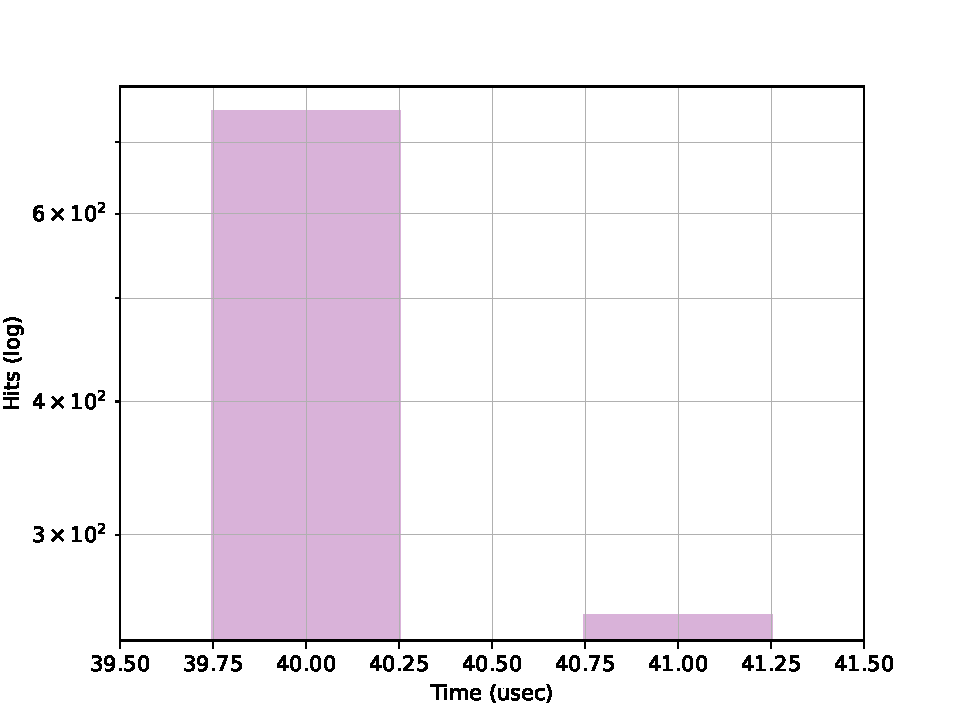
\includegraphics[scale=.4]{assets/extension-framework-riot-z1.pdf}
      \caption{Extension framework distribution with RIOT on Z1\label{fig:extension-framework-riot-z1}}
  \end{minipage}
\end{figure}

\subsection{Discussion}

To discuss the results, we first compare them with our reference value.
This will allow us to determine if our framework measurements are correct.
Then, we will explain those results.

\subsubsection{Comparisons}

\begin{figure}[!ht]
  \begin{minipage}{.45\textwidth}
      \centering
      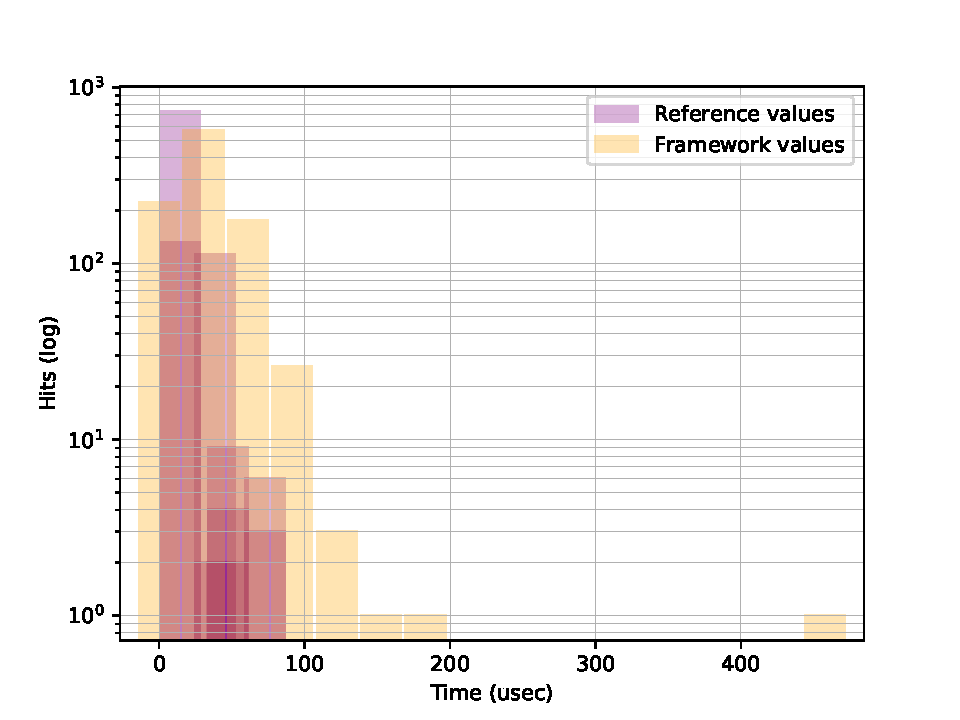
\includegraphics[scale=.4]{assets/comparison-extension-framework-contiki-remote.pdf}
      \caption{Extension framework evaluation with Contiki on RE-Mote\label{fig:comparison-extension-framework-contiki-remote}}
  \end{minipage}\hfill
  \begin{minipage}{.45\textwidth}        
      \centering
      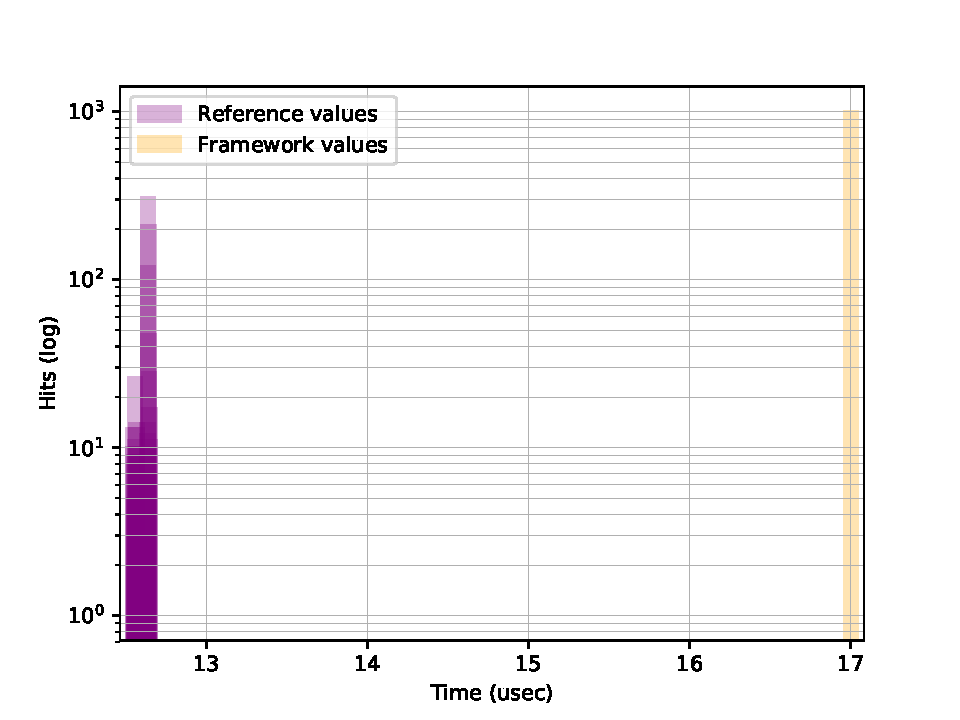
\includegraphics[scale=.4]{assets/comparison-extension-framework-riot-remote.pdf}
      \caption{Extension framework evaluation with RIOT on RE-Mote\label{fig:comparison-extension-framework-riot-remote}}
  \end{minipage}
\end{figure}

\begin{figure}[!ht]
  \begin{minipage}{.45\textwidth}
      \centering
      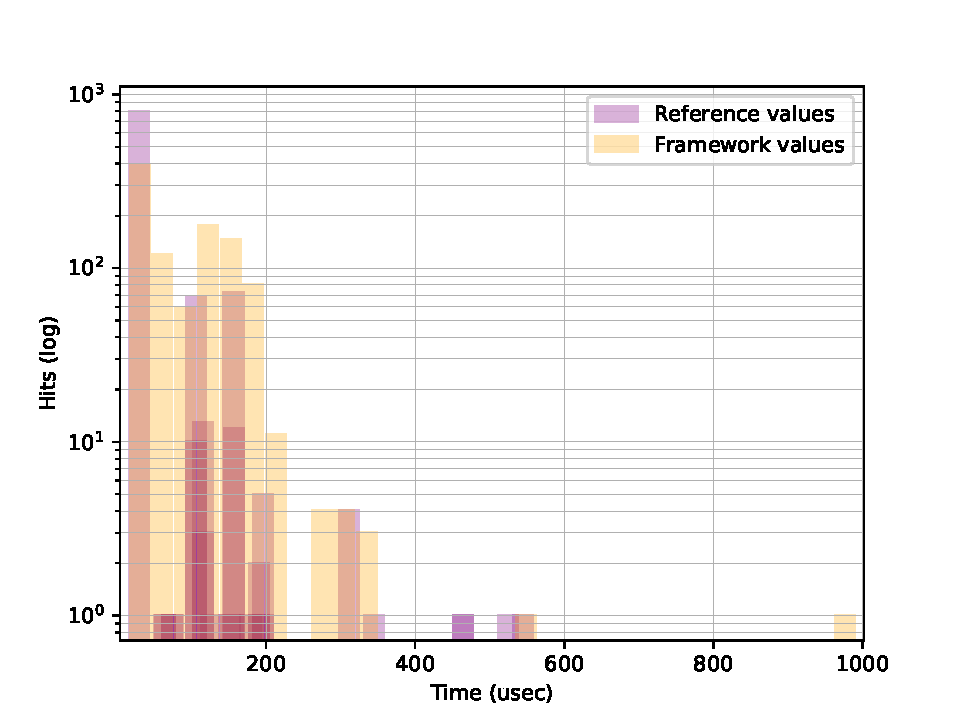
\includegraphics[scale=.4]{assets/comparison-extension-framework-contiki-z1.pdf}
      \caption{Extension framework evaluation with Contiki on Z1\label{fig:comparison-extension-framework-contiki-z1}}
  \end{minipage}\hfill
  \begin{minipage}{.45\textwidth}        
      \centering
      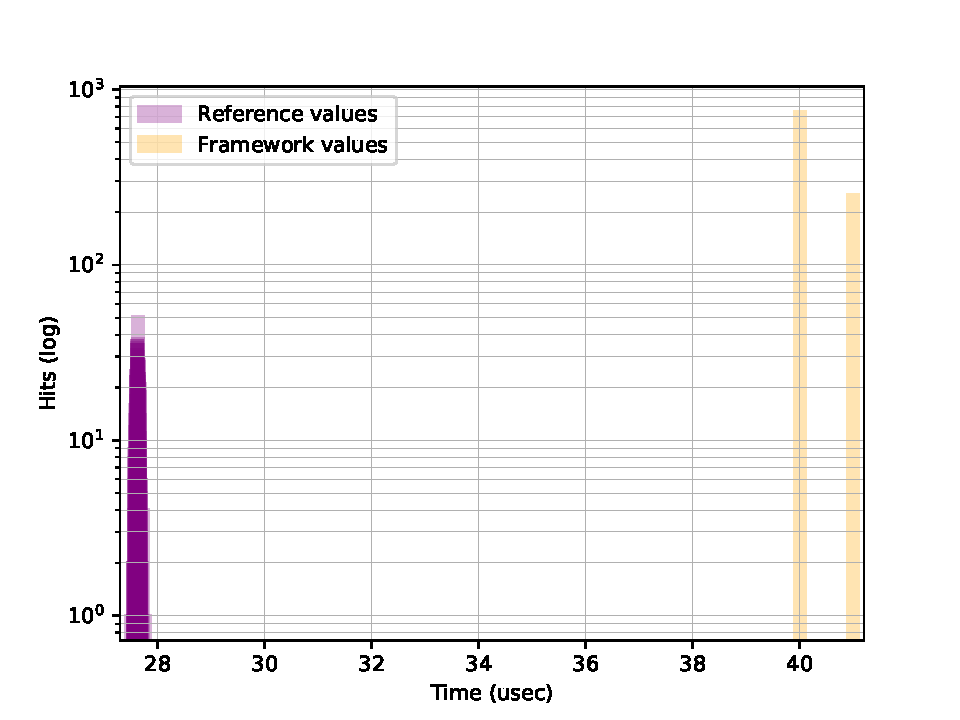
\includegraphics[scale=.4]{assets/comparison-extension-framework-riot-z1.pdf}
      \caption{Extension framework evaluation with RIOT on Z1\label{fig:comparison-extension-framework-riot-z1}}
  \end{minipage}
\end{figure}

\subsubsection{Limitation of the framework}
As the results show, our extension framework is not able to compute the context switching time of our simple application.
The devices do not have enough precision with their real-time clock.